\chapter{Descrição da técnica}

A técnica usada neste trabalho é baseada em arestas e usa um modelo pré-definido para a pose inicial. A extração das arestas é feita por amostragem de pontos, descrita na seção anterior.

\begin{comment}
\section{Trabalhando com múltiplas hipóteses}

Um dos problemas que ocorrem nas técnicas \emph{edge-based} é que nem sempre se consegue extrair com precisão as arestas da imagem. Na seção anterior foi discutido que um dos passos para a extração das arestas é a procura por pontos de alto gradiente na normal da aresta. Muitas vezes é possível encontrar vários desses pontos para cada amostra, e neste caso obtém-se múltiplas hipóteses de pontos da imagem correspondente ao ponto amostrado. Veja a \figref{cubo_0}.

%O que se faz neste caso é, para cada aresta do modelo, trabalhar com múltiplos correspondentes na imagem.

%Como existem múltiplas hipóteses de correspondência em cada amostra do modelo, pode-se concluir que existirão múltiplas hipóteses de arestas para compor a pose da cena atual, como mostra a \figref{cubo_0}

O trabalho com múltiplas hipóteses foi inicialmente proposto em \cite{multiplas_hipoteses}. Neste trabalho cada aresta $E_i$ (do modelo) projetada na imagem tem um conjunto $\{e_{i,j}\}$ de pontos amostrados. Cada ponto $e_{i,j}$ tem um conjunto $\{e'_{i,j,l}\}$ de hipóteses de correspondência. Em \cite{multiplas_hipoteses} a hipótese $e'_{i,j,l}$ é aquela que tem a menor distância da aresta projetada $E_i$. Então mesmo que sejam encontrados pontos de forte gradiente na normal da aresta $E_i$, aquele que mais se aproxima da aresta projetada é escolhido como correspondente a $e_{i,j}$. Tendo este conjunto de correspondências, o processo continua como no caso de hipótese única.
\end{comment}

Na técnica de múltiplas hipóteses um dos candidatos é escolhido para ser associado com a amostra do modelo, no caso, o candidato mais próximo da aresta projetada. Entretanto isso nem sempre resulta na melhor pose final, pois outros pontos de forte gradiente, como objetos externos ou até uma outra aresta do próprio objeto, podem confundir todo o cálculo da pose só porque estão mais próximos de uma determinada aresta do modelo. Isso pode ser visualizado na \figref{multiplas_hipoteses_errada}, em que além da aresta do objeto, o lápis também é identificado pelo algoritmo de busca. O fato de uma das arestas do modelo projetado estar mais perto do lápis do que do próprio objeto faz com que o algoritmo de rastreamento o utilize como aresta do objeto e faça o cálculo de pose a partir disso, o que vai fazer uma grande diferença no processo de rastreamento a partir de então. Uma forma de contornar essa situação seria também escolher outras hipóteses (não somente a mais próxima) e calcular novas poses a partir de diferentes agrupamentos amostra-hipótese. O trabalho \cite{celine} propõe exatamente isso: que sejam calculadas diversas poses, utilizando hipóteses diferentes, para que no final as poses calculas sejam comparadas e a melhor dentre elas seja escolhida.

\begin{figure}[!ht]
\centering\includegraphics{monografia/multiplas_hipoteses_errada}
\caption{Casamento de hipóteses errado. O algoritmo encontrou múltiplas hipóteses para as amostras, mas optou por casar com as hipóteses erradas porque estavam mais próximas.}
\label{multiplas_hipoteses_errada}
\end{figure}

Um dos principais passos do algoritmo visa fazer combinações de agrupamento amostra-hipótese, pois combinar todos os possíveis casamentos amostra-hipótese não é uma estratégia válida, já que isso pode significar o cálculo de milhares de poses por cada \emph{frame}, mesmo que o objeto rastreado seja simples, como um cubo. Um outro problema de se fazer todas as possíveis combinações é que nem sempre um agrupamento de hipóteses revela uma possível aresta do objeto. Na \figref{agrupamento_errado_de_hipoteses} temos as amostras (em vermelho) e suas respectivas hipóteses (quadrados). A \figref{agrupamento_errado_de_hipoteses} exemplifica um caso de um casamento qualquer de amostras e hipóteses em que as hipóteses escolhidas estão em verde. A escolha dessas hipóteses claramente não resultaria em uma pose válida, pois o sistema iria tentar convergir uma de suas arestas (a com amostras vermelhas) para os pontos marcados em verde, e isso estaria longe de uma pose válida. Como o algoritmo trabalha com múltiplas hipóteses de pose, a pose gerada pela \figref{agrupamento_errado_de_hipoteses} provavelmente seria descartada em um passo posterior, mas é melhor evitar esse tipo de agrupamento para que sejam feitos menos cálculos de pose desnecessários. \cite{celine} sugere que se façam agrupamentos que sejam o mais próximo possível de uma reta, como exemplificado na \figref{agrupamento_certo_de_hipoteses}. Seguindo essa estratégia pode-se dizer que a abordagem trabalha não com múltiplas hipóteses de pontos do objeto, mas com múltiplas hipóteses de aresta. Veja a \figref{hipoteses_de_aresta}.

\begin{figure}[!ht]
\centering\includegraphics{monografia/agrupamento_errado_de_hipoteses}
\caption{Hipóteses agrupadas sem formar uma linha. Os pontos vermelhos são as amostras do modelo; os quadrados são as hipóteses de cada amostras; os quadrados de cor verde são as hipóteses escolhidas.}
\label{agrupamento_errado_de_hipoteses}
\end{figure}

\begin{figure}[!ht]
\centering\includegraphics{monografia/agrupamento_certo_de_hipoteses}
\caption{A figura mostra dois tipos agrupamentos (um rosa e outro verde) de modo que se aproximem de uma linha. Esse tipo de agrupamento é mais próximo de uma aresta que o mostrado na \figref{agrupamento_errado_de_hipoteses}}
\label{agrupamento_certo_de_hipoteses}
\end{figure}

\begin{figure}[!ht]
\centering\includegraphics{monografia/hipoteses_de_aresta}
\caption{A figura mostra dois tipos de agrupamento (um rosa e outro verde) formando duas hipóteses de aresta de mesma cor.}
\label{hipoteses_de_aresta}
\end{figure}

O uso de múltiplas hipóteses de aresta simplifica o trabalho de agrupar múltiplas hipóteses para se calcular novas poses. No caso, basta selecionar uma hipótese de aresta para cada aresta visível do modelo que já é possível calcular uma nova pose que projeta o modelo o mais próximo possível das arestas escolhidas.

% TODO: cálculo do erro

Em poucas palavras o algoritmo se resume a:

\begin{itemize}
	\item Projetar o modelo usando a pose do quadro anterior;
	\item Amostrar as arestas do modelo projetado;
	\item Fazer uma busca por pontos de forte gradiente na normal de cada amostra. Esses pontos serão as hipóteses da amostra;
	\item Em cada aresta, criar grupos de hipóteses de modo que não existam duas hipóteses em um mesmo grupo que pertençam à mesma amostra. Esses grupos devem aproximar, da melhor forma possível, seus elementos de uma reta;
	\item Para cada aresta visível do modelo, escolher uma de suas hipóteses de aresta e calcular a pose que projeta o modelo o mais próximo possível das arestas selecionadas. Observe que a escolha das hipóteses de aresta seguido do cálculo da pose se assemelha bastante à técnica de extração explícita de aresta, visto na seção \ref{sec:extracao_explicita};
	\item Repetir o passo anterior tantas vezes quanto forem a quantidade de poses necessárias;
	\item Avaliar o erro de cada pose calculada e escolher a que possuir o menor erro de reprojeção.
\end{itemize}

\section{Extraindo a hipótese de aresta}

As hipóteses de aresta são formadas agrupando $k_i$ conjuntos de $e'_{i,j,l}$ (uma das hipóteses da amostra $e_{i,j}$, como mostra a \figref{multiplas_hipoteses_celine}) e extraindo a reta que mais se aproxima desse conjunto de pontos. O número $k_i$ de conjuntos é dado pelo maior número de hipóteses detectadas por uma amostra da aresta $E_i$, ou seja $k_i = max_j\{n_{i,j}\}$, sendo $n_{i,j}$ o número de candidatos associados à amostra $e_{i,j}$.

\begin{figure}[!ht]
\centering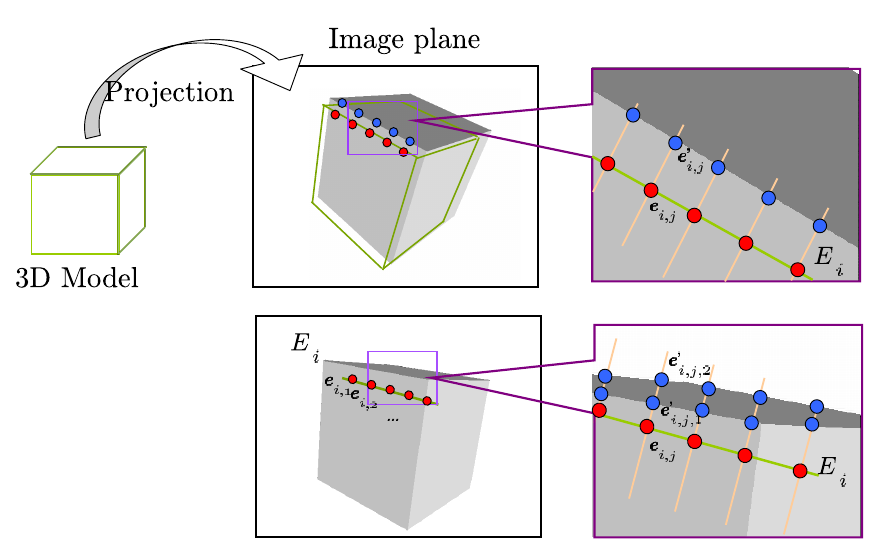
\includegraphics[width=0.9\textwidth]{monografia/multiplas_hipoteses_celine}
\caption{Visualização das múltiplas hipóteses. Figura retirada de \cite{celine}.}
\label{multiplas_hipoteses_celine}
\end{figure}

Para formar esses conjuntos, as hipóteses $e'_{i,j,l}$ de cada aresta são agrupadas utilizando um algoritmo de classificação \emph{k-means}. Para cada aresta $E_i$, o algoritmo agrupa as hipóteses de pontos $e'_{i,j,l}$ em $k_i$ conjuntos (ou classes), que será chamada de $(c^i_1, \dots, c^i_{k_i})$. O centróide de cada classe é a reta resultante do algoritmo \emph{fitline} \cite{fitline_doc} com o conjunto de pontos da classe.

Inicialmente as hipóteses $e'_{i,j,l}$ da aresta $E_i$ são agrupadas nas classes $(c^i_1, \dots, c^i_{k_i})$ na ordem em que elas foram encontradas na busca pela normal. Dessa forma a classe $c^i_m$ é formada inicialmente pelo conjunto $\{e'_{i,j,m}\}$, em que $0 < j \leq n_i$ e $n_i$ é o número de amostras da aresta $E_i$. Esse é um bom agrupamento inicial, já que boa parte das amostras já estão localizadas no seu \emph{cluster} final. Em seguida são calculadas as distâncias de cada hipótese $e'_{i,j,l}$ da amostra $e_{i,j}$ para cada um dos centróides $(c^i_1, \dots, c^i_{k_i})$. Esse cálculo de distâncias serve para realocar as hipóteses para os \emph{clusters} mais próximos.

No trabalho original \cite{celine} é dito que esse último passo seja repetido até que não haja mais trocas entre os \emph{clusters}, mas na prática precisou-se estabelecer um número máximo de iterações, pois muitas vezes o algoritmo repetia indefinidamente.

% TODO: Esses passos são melhor explicados no algoritmo abaixo.

Ao final das iterações a aresta $E_i$ possui um conjunto de \emph{clusters} $c^i_m = (\{e'_{i,j,m}\}, r^i_m)$, sendo que $r^i_m$ é descrito na equação.

\begin{equation}
r^i_m = \frac{1}{N} \sum^{N}_{j = 0} \Delta (e'_{i,j,m}, c^i_m)
\end{equation}

em que $N$ é o número de elementos do \emph{cluster} $c^i_m$, e $\Delta (e', c)$ é a função que calcula a distância do ponto $e'$ à reta $c$. O resíduo $r^i_m$ será usado para a próxima seção.

\section{Obtendo as hipóteses de pose}

Após extrair as hipóteses de aresta, as hipóteses de pose são obtidas ao se escolher, para cada aresta $E_i$, uma classe $c^i_{p_i}$. A escolha é feita de forma aleatória, mas considerando o peso $w^i_m$ de cada hipótese de aresta.

O peso $w^i_m$ é deduzido pela equação:

\begin{equation}
w^i_m = \begin{cases}
    e^{-\lambda \left( \frac{r^i_m - r^i_{min}}{r^i_{max} - r^i_{min}}\right)^2 } & \mbox{se } r^i_{max} \neq r^i_{min} \\
    1 & \mbox{senão}.
\end{cases}
\end{equation}

em que $\lambda$ é um parâmetro que pode ser ajustado.

Faz-se uma escolha aleatória com pesos para que todas as hipóteses de aresta tenham chance de serem escolhidas para formar uma pose, embora as arestas de maior peso tenham mais chances de serem escolhidas.

Após isso é calculado o erro de reprojeção de cada pose formada. A que possuir menor erro é considerada a pose da cena atual e será usada para as próximas iterações do algoritmo.

\begin{comment}
\section{Rascunho}

\begin{figure}[ht!]
\centering
\includegraphics{monografia/cubo_arestas}
\caption{}
\label{cubo_arestas}
\end{figure}

A \figref{cubo_arestas} ilustra que as hipóteses de aresta são extraídas a partir das hipóteses das amostras. A escolha das arestas foi feita de maneira que para cada amostra escolhida, a primeira hipótese encontrada irá compor a primeira aresta; a segunda hipótese fará parte da segunda aresta e assim por diante.

\begin{figure}[ht!]
\centering
\includegraphics{monografia/cubo_kmeans}
\caption{}
\label{cubo_kmeans}
\end{figure}

No algoritmo usado nesse trabalho, baseado em \cite{celine}, é feita uma clusterização usando \emph{k-means} para que as hipóteses fiquem o mais próximo possível das arestas formadas. Como ilustrado na \figref{cubo_kmeans}, as hipóteses da \figref{cubo_arestas} são realocadas para que cada conjunto hipóteses forme um \emph{cluster} (ou aresta).

\section{Escolha da pose}

Para cada aresta da pose anterior, uma das hipóteses de aresta é escolhida aleatoriamente e assim será formada a pose atual.
\end{comment}

\begin{comment}
\section{A FAZER}

\begin{enumerate}
\item Descrever o moving-edges. Mostrar que com múltiplas hipóteses a $n$-ésima hipótese de ponto vai corresponder à $n$-ésima hipótese de aresta.
\item Falar sobre \cite{celine}. As hipóteses de pontos vão formar arestas tal que elas fiquem as mais paralelas possíveis da aresta da cena atual.
\item colocar figuras para ilustrar
\end{enumerate}
\end{comment}
